\section{Riihitykset Piilopirtillä}

\textit{Rusakoiden vanhempien ikäkausien yhä seuraamat 
luokkamerkkivaatimukset ovat lippukunnan oma sovellus perinteisistä 
suomalaisista partio"-ohjelmista. Luokkamerkkien avulla opitaan monia 
hyödyllisiä erätaitoja ja tutustutaan partiotapoihin. Luokkamerkin 
loppukokeessa eli riihityksessä päästään soveltamaan opittuja taitoja 
käytännössä.}

\textit{Viimeksi riihityksiä on järjestetty Sipoonkorvessa 12.4.2025, 
Länsi"-Helsingissä 9.6.2019 ja Nuuksiossa 10.2.2018. Tässä jutussa 
päästään kurkistamaan niin sanotusti esiripun taakse, kun julkaisemme 
vuoden 2018 riihityksenaikaisen rastimiesten Whatsapp"-ryhmän keskustelun. 
A"-Team"-vartio teki Lentävä nuoli "=merkkiin liittyviä rastitehtäviä, kun 
taas Jamalit 5000 ja Suunnistajat"-vartiot suorittivat III luokkaa ja 
Unibrows"-vartio II luokkaa. Julkaisemme myös Unibrows"-vartion kirjoittaman 
riihitysraportin ensimmäistä kertaa.}

\medskip

\noindent\null\hfill Kuva ja teksti: Janne

\begin{multicols}{2}
\setlength{\parindent}{0em} 10.59 - V: A-team matkalla! (J: ilmoita myös 
kumpaa puolta Orajärveä 2:lta lähdetään)

11.02 - V: Jamalit 5000 lähtee, tai ainakin kovasti yrittää...

11.04 - V: Suunnistajat lähtee

11.08 - V: Ja viimeisetkin matkaan!

11.29 - T: Rastimies 1 asemissa, ryhmästä X näkö- ja äänihavainto 
toiselta rannalta

11.46 - J: Rastimies 2 matkalla: etappi 1-2 erit. raskas. ~30 cm lunta, ei 
tallottu...

11.48 - T: Ryhmä 1 poistui rastilta 2

11.51 - J: Suunnistajat hukassa. Soittivat. Ovat ilmeisesti Ruuhijärven 
rannassa...

11.52 - T: Taisivat minulle koittaa kanssa, en ehtinyt vastata. Muut 
rastilla/matkalla rastille 2

12.08 - J: Rasti 2 asemissa.

12.12 - V: Rastia 4 vielä etsitään, eli 3:lle ei kannata ketään 
päästää...

12.19 - T: Viimeinen ryhmä saapui rastille 1, vahvuus vain 3, yksi puuttuu

12.22 - T: Ryhmä siis suunnistajat, K ilmeisesti palannut kämpälle, tai 
ainakin sinne suuntaan lähtenyt

12.33 - T: Viimeinen ryhmä poistui rastilta 1, rastimies aloittaa siirtymän 
kohti rastia 5

12.36 - J: Onko rasti 3 asemissa?

12.36 - V: Ei, vielä ei edes 4 löytynyt...

12.38 - J: A-Team lähtövalmiudessa rastilla 2. Odottaa lähtölupaa...

12.46 - M: Rasti 4 on miehitetty. Täällä on korppi!

12.51 - J: Jamalit 5000 lähtövalmiudessa rastilla 2. Odottaa lähtölupaa...

13.05 - J: Unibrows lähtövalmiudessa rastilla 2. Odottaa lähtölupaa...

\begin{figure*}[!t]
\centering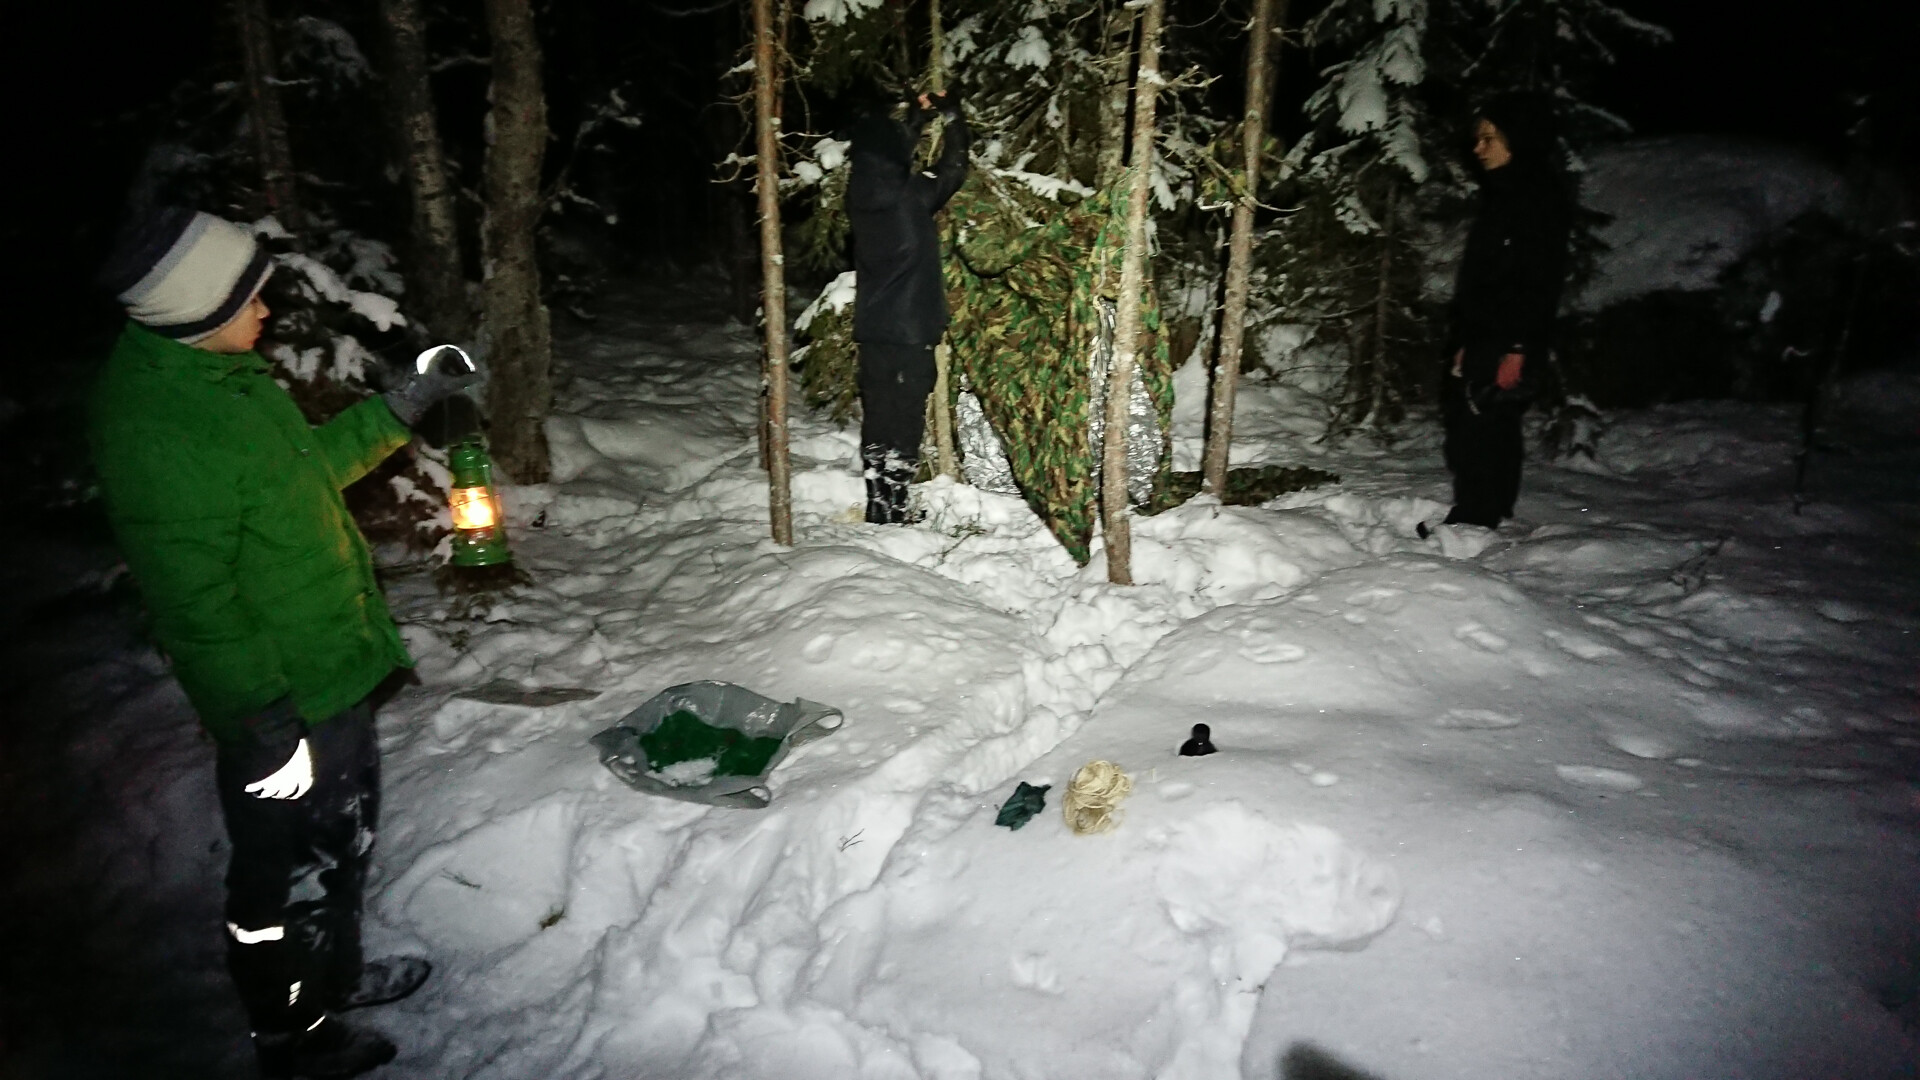
\includegraphics[width=\textwidth,trim={0 0 0 .15cm},clip]{assets/riihitys2018}
\caption{Unibrows"-vartio riihityksen viimeisellä rastilla kasaamassa myrskylyhtyä ja 
laavua.}
\end{figure*}

13.09 - T: Ruokarastille saavuttu, eksynyt lammas seisoi kuistilla. Jätin 
siihen.

13.11 - V: Käännyn nyt ladulta (lähes umpinaiselle) polulle kohti 3, voi 
laittaa ryhmiä yksi kerrallaan liikkeelle...

13.13 - J: A-Team lähti rastilta 2. Orajärven itälaitaa.

13.17 - J: Jamalit 5000 lähti rastilta 2. Orajärven itälaitaa.

13.21 - J: Unibrows lähti rastilta 2. Orajärven itälaitaa.

13.41 - J: Suunnistajat lähti rastilta 2. Orajärven itälaitaa.

13.42 - J: Kaikki käyneet rastilla 2. Rasti sulkeutuu.

13.42 - M: {\fontspec{Symbola}\symbol{"1F44D}}

14.09 - V: Rasti 3 paikallaan, Jamalit 5000 ja A-team jatkavat kohti rastia 4

14.26 - M: XXX on kadonneiden ryhmien numero... J5000 ja AAA omien sanojensa 
mukaan hukassa...

14.27 - M: Ovat siis yhdessä.

14.27 - V: Unibrows lähti rastilta 3, myös Suunnistajien ääni kuultu 
(muttei vielä näköhavaintoa)...

14.41 - J: Unibrows löydetty.

14.43 - J: AAAn ja J5000 kaukainen äänihavainto.

14.44 - M: Upeeta! Pyysin heitä pitämään älämölöä...

14.53 - J: Siis toso kaukainen. +1 km.

14.54 - V: Suunnistajat melkein rastilla 4, lähden täältä yhtä matkaa 
ryhmän kanssa niin eivät eksy...

14.55 - M: Kuulin huudon itsestäni koilliseen.

14.59 - J: Vartiot löydetty

15.00 - M: {\fontspec{Symbola}\symbol{"1F44D}}

15.10 - J: Aika nuutunutta on porukka. 4. rastille 950 m linnuntietä.

15.21 - J: Unibrows saatu kiinni. Nyt on 3 vartiota klimpissä.

15.49 - M: AAA ja J5000 lähtivät kämpälle tie -reittiä.

15.50 - M: Unibrows ei ole saapunut vielä rastille 4.

15.50 - M: Myös suunistajia odotellaan...

15.50 - V: Suunnistajat kääntyvät juuri ladulta pohjoiseen kohti rastia 4

15.52 - M: Huolestummeko Unibrowsista?

16.00 - V: Unibrowskin löysi tiensä rastille 4...

16.01 - V: T: voisit laittaa kuumaa mehua valmiiksi, täällä aika 
paleltunutta ja väsynyttä poukkaa tulossa...

16.05 - T: Laitetaan. Myös takka sytytettiin, että kämppään saadaan 
vähän lämpöä.

16.07 - J: AAA maalissa.

16.14 - J: J5000 maalissa.

16.19 - M: Unibrows has left the 4th piste.

19.06 - M: A:lla on huoltoaluepalvelua. Sen kengät on katastrofi...
\end{multicols}

\medskip

\noindent\textbf{Unibrows"-vartion riihitysraportti}

\begin{multicols}{2}
\noindent Aloittaessamme riihitystä meille ilmeni heti pienoinen ongelma, 
sillä kukaan meistö ei oikein muistanut kuinka kartasta katsotaan 
koordinaatteja. Lopulta pääsimme lähtemään ensimmäiselle rastille päin. 
Ensimmäisellä rastilla testattiin tietämystämme ilmansuunnista (esim. mihin 
päin muurahaiskeko osoittaa). Tämän jälkeen arvioimme erilaisia pituuksia. 
Toisella Rastilla kertasimme, että miten joku pelastetaan jäistä. tämän 
jälkeen odotimme hetken aikaa, että Väinö olisi omalla rastillaan. 
Lähtiessämme kolmannelle rastille oli se jo raskasta, sillä maasto oli jo 
muuttumassa korkeaksi. Lähtiessämme kolmannelta rastilta olimme jo poikki, ja 
eksyimme hieman matkalla. Lopulta pääsimme perille, mutta olimme kaikki 
kylmissään ja juuri silloin meidän piti ruveta tekemään solmuja 
(paalusolmu ja pukkisolmu jos oikein muistan). palatessamme piilopirtille muut 
olivat jo kokkaamassa ruokaa. Liityimme heihin ja rupesimme myöskin 
kokkaamaan. Ruokamme kylläkin paloi pahasti pohjaan, mutta hyvää se silti 
oli. Viimeisen rastin suoritimme pimeässä, ja silloin pystytimme laavun 
sillä aikaa, kun Miika kokosi myrskylyhtyä jonka Janne oli hänelle purkanut. 
Saatuamme Jonnin kanssa laavun pystytettyä ja purettua, aloitimme viimeisen 
rastin. Rastin tehtävänä oli, että me suunnistamme takaisin piilopirtille. 
MUTTA me emme saaneet käyttää samoja polkuja joita olimme jo käyttäneet. 
Rämmimme sitten siellä metässä jonkin verran mutta pääsimme lopulta 
takaisin piilopirtille. 
\end{multicols}

\medskip

\noindent\null\hfill Teksti: Ilari
